% Created by tikzDevice version 0.12.6 on 2026-08-08 12:11:52
% !TEX encoding = UTF-8 Unicode
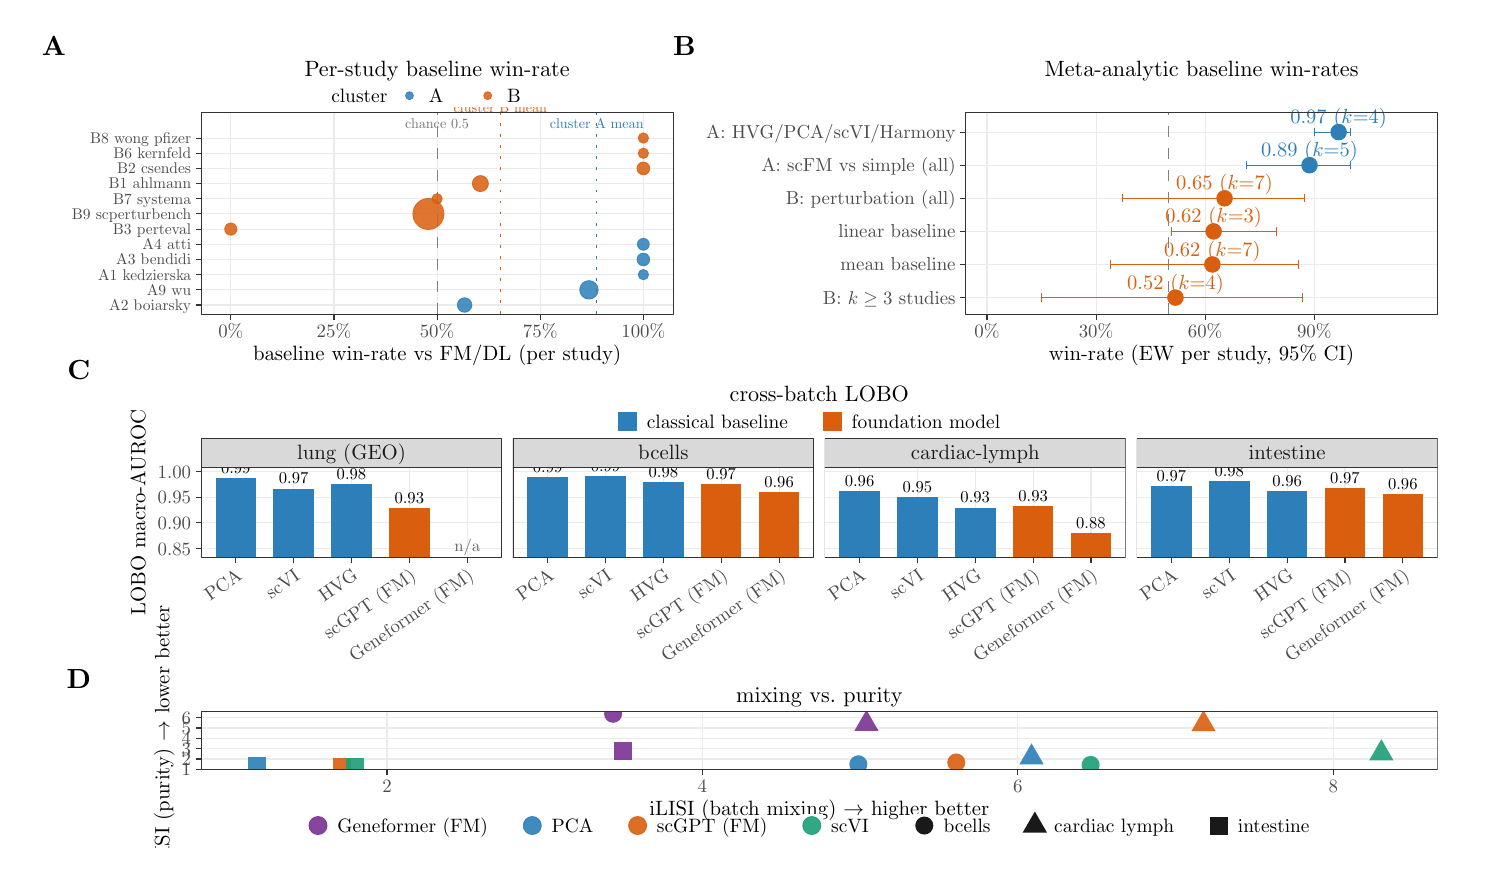
\begin{tikzpicture}[x=1pt,y=1pt]
\definecolor{fillColor}{RGB}{255,255,255}
\path[use as bounding box,fill=fillColor,fill opacity=0.00] (0,0) rectangle (517.45,296.31);
\begin{scope}
\path[clip] (  0.00,  0.00) rectangle (517.45,296.31);
\definecolor{drawColor}{RGB}{255,255,255}
\definecolor{fillColor}{RGB}{255,255,255}

\path[draw=drawColor,line width= 0.4pt,line join=round,line cap=round,fill=fillColor] (  0.00,  0.00) rectangle (517.45,296.31);
\end{scope}
\begin{scope}
\path[clip] (  8.00, 63.91) rectangle (513.45,172.57);
\definecolor{drawColor}{RGB}{255,255,255}
\definecolor{fillColor}{RGB}{255,255,255}

\path[draw=drawColor,line width= 0.4pt,line join=round,line cap=round,fill=fillColor] (  8.00, 63.91) rectangle (513.45,172.57);
\end{scope}
\begin{scope}
\path[clip] (  8.00,  2.00) rectangle (513.45, 63.91);
\definecolor{drawColor}{RGB}{255,255,255}
\definecolor{fillColor}{RGB}{255,255,255}

\path[draw=drawColor,line width= 0.4pt,line join=round,line cap=round,fill=fillColor] (  8.00,  2.00) rectangle (513.45, 63.91);
\end{scope}
\begin{scope}
\path[clip] (  8.00,172.57) rectangle (237.21,290.31);
\definecolor{drawColor}{RGB}{255,255,255}
\definecolor{fillColor}{RGB}{255,255,255}

\path[draw=drawColor,line width= 0.4pt,line join=round,line cap=round,fill=fillColor] (  8.00,172.57) rectangle (237.21,290.31);
\end{scope}
\begin{scope}
\path[clip] (237.21,172.57) rectangle (513.45,290.31);
\definecolor{drawColor}{RGB}{255,255,255}
\definecolor{fillColor}{RGB}{255,255,255}

\path[draw=drawColor,line width= 0.4pt,line join=round,line cap=round,fill=fillColor] (237.21,172.57) rectangle (513.45,290.31);
\end{scope}
\begin{scope}
\path[clip] (  0.00,  0.00) rectangle (517.45,296.31);
\definecolor{fillColor}{RGB}{255,255,255}

\path[fill=fillColor] ( 62.66,192.80) rectangle (233.21,265.74);
\definecolor{drawColor}{gray}{0.92}

\path[draw=drawColor,line width= 0.4pt,line join=round] ( 62.66,196.09) --
	(233.21,196.09);

\path[draw=drawColor,line width= 0.4pt,line join=round] ( 62.66,201.57) --
	(233.21,201.57);

\path[draw=drawColor,line width= 0.4pt,line join=round] ( 62.66,207.06) --
	(233.21,207.06);

\path[draw=drawColor,line width= 0.4pt,line join=round] ( 62.66,212.54) --
	(233.21,212.54);

\path[draw=drawColor,line width= 0.4pt,line join=round] ( 62.66,218.03) --
	(233.21,218.03);

\path[draw=drawColor,line width= 0.4pt,line join=round] ( 62.66,223.51) --
	(233.21,223.51);

\path[draw=drawColor,line width= 0.4pt,line join=round] ( 62.66,229.00) --
	(233.21,229.00);

\path[draw=drawColor,line width= 0.4pt,line join=round] ( 62.66,234.48) --
	(233.21,234.48);

\path[draw=drawColor,line width= 0.4pt,line join=round] ( 62.66,239.97) --
	(233.21,239.97);

\path[draw=drawColor,line width= 0.4pt,line join=round] ( 62.66,245.45) --
	(233.21,245.45);

\path[draw=drawColor,line width= 0.4pt,line join=round] ( 62.66,250.93) --
	(233.21,250.93);

\path[draw=drawColor,line width= 0.4pt,line join=round] ( 62.66,256.42) --
	(233.21,256.42);

\path[draw=drawColor,line width= 0.4pt,line join=round] ( 73.40,192.80) --
	( 73.40,265.74);

\path[draw=drawColor,line width= 0.4pt,line join=round] (110.67,192.80) --
	(110.67,265.74);

\path[draw=drawColor,line width= 0.4pt,line join=round] (147.94,192.80) --
	(147.94,265.74);

\path[draw=drawColor,line width= 0.4pt,line join=round] (185.21,192.80) --
	(185.21,265.74);

\path[draw=drawColor,line width= 0.4pt,line join=round] (222.48,192.80) --
	(222.48,265.74);
\definecolor{drawColor}{gray}{0.50}

\path[draw=drawColor,line width= 0.4pt,dash pattern=on 4pt off 4pt ,line join=round] (147.94,192.80) -- (147.94,265.74);
\definecolor{drawColor}{RGB}{44,127,184}

\path[draw=drawColor,line width= 0.4pt,dash pattern=on 1pt off 3pt ,line join=round] (205.62,192.80) -- (205.62,265.74);
\definecolor{drawColor}{RGB}{217,95,14}

\path[draw=drawColor,line width= 0.4pt,dash pattern=on 1pt off 3pt ,line join=round] (170.79,192.80) -- (170.79,265.74);
\definecolor{drawColor}{gray}{0.45}

\node[text=drawColor,anchor=base,inner sep=0pt, outer sep=0pt, scale=  0.51] at (147.94,259.95) {chance 0.5};
\definecolor{drawColor}{RGB}{44,127,184}

\node[text=drawColor,anchor=base,inner sep=0pt, outer sep=0pt, scale=  0.51] at (205.62,259.95) {cluster A mean};
\definecolor{drawColor}{RGB}{217,95,14}

\node[text=drawColor,anchor=base,inner sep=0pt, outer sep=0pt, scale=  0.51] at (170.79,265.59) {cluster B mean};
\definecolor{drawColor}{RGB}{44,127,184}
\definecolor{fillColor}{RGB}{44,127,184}

\path[draw=drawColor,draw opacity=0.85,line width= 0.3pt,line join=round,line cap=round,fill=fillColor,fill opacity=0.85] (222.48,207.06) circle (  1.87);

\path[draw=drawColor,draw opacity=0.85,line width= 0.3pt,line join=round,line cap=round,fill=fillColor,fill opacity=0.85] (157.88,196.09) circle (  2.62);

\path[draw=drawColor,draw opacity=0.85,line width= 0.3pt,line join=round,line cap=round,fill=fillColor,fill opacity=0.85] (222.48,212.54) circle (  2.28);

\path[draw=drawColor,draw opacity=0.85,line width= 0.3pt,line join=round,line cap=round,fill=fillColor,fill opacity=0.85] (222.48,218.03) circle (  2.15);

\path[draw=drawColor,draw opacity=0.85,line width= 0.3pt,line join=round,line cap=round,fill=fillColor,fill opacity=0.85] (202.81,201.57) circle (  3.34);
\definecolor{drawColor}{RGB}{217,95,14}
\definecolor{fillColor}{RGB}{217,95,14}

\path[draw=drawColor,draw opacity=0.85,line width= 0.3pt,line join=round,line cap=round,fill=fillColor,fill opacity=0.85] (163.58,239.97) circle (  2.90);

\path[draw=drawColor,draw opacity=0.85,line width= 0.3pt,line join=round,line cap=round,fill=fillColor,fill opacity=0.85] (222.48,245.45) circle (  2.31);

\path[draw=drawColor,draw opacity=0.85,line width= 0.3pt,line join=round,line cap=round,fill=fillColor,fill opacity=0.85] ( 73.40,223.51) circle (  2.20);

\path[draw=drawColor,draw opacity=0.85,line width= 0.3pt,line join=round,line cap=round,fill=fillColor,fill opacity=0.85] (222.48,250.93) circle (  1.87);

\path[draw=drawColor,draw opacity=0.85,line width= 0.3pt,line join=round,line cap=round,fill=fillColor,fill opacity=0.85] (147.94,234.48) circle (  1.87);

\path[draw=drawColor,draw opacity=0.85,line width= 0.3pt,line join=round,line cap=round,fill=fillColor,fill opacity=0.85] (222.48,256.42) circle (  1.87);

\path[draw=drawColor,draw opacity=0.85,line width= 0.3pt,line join=round,line cap=round,fill=fillColor,fill opacity=0.85] (144.81,229.00) circle (  5.61);
\definecolor{drawColor}{gray}{0.20}

\path[draw=drawColor,line width= 0.4pt,line join=round,line cap=round] ( 62.66,192.80) rectangle (233.21,265.74);
\end{scope}
\begin{scope}
\path[clip] (  0.00,  0.00) rectangle (517.45,296.31);
\definecolor{drawColor}{gray}{0.30}

\node[text=drawColor,anchor=base east,inner sep=0pt, outer sep=0pt, scale=  0.56] at ( 59.06,194.16) {A2 boiarsky};

\node[text=drawColor,anchor=base east,inner sep=0pt, outer sep=0pt, scale=  0.56] at ( 59.06,199.65) {A9 wu};

\node[text=drawColor,anchor=base east,inner sep=0pt, outer sep=0pt, scale=  0.56] at ( 59.06,205.13) {A1 kedzierska};

\node[text=drawColor,anchor=base east,inner sep=0pt, outer sep=0pt, scale=  0.56] at ( 59.06,210.61) {A3 bendidi};

\node[text=drawColor,anchor=base east,inner sep=0pt, outer sep=0pt, scale=  0.56] at ( 59.06,216.10) {A4 atti};

\node[text=drawColor,anchor=base east,inner sep=0pt, outer sep=0pt, scale=  0.56] at ( 59.06,221.58) {B3 perteval};

\node[text=drawColor,anchor=base east,inner sep=0pt, outer sep=0pt, scale=  0.56] at ( 59.06,227.07) {B9 scperturbench};

\node[text=drawColor,anchor=base east,inner sep=0pt, outer sep=0pt, scale=  0.56] at ( 59.06,232.55) {B7 systema};

\node[text=drawColor,anchor=base east,inner sep=0pt, outer sep=0pt, scale=  0.56] at ( 59.06,238.04) {B1 ahlmann};

\node[text=drawColor,anchor=base east,inner sep=0pt, outer sep=0pt, scale=  0.56] at ( 59.06,243.52) {B2 csendes};

\node[text=drawColor,anchor=base east,inner sep=0pt, outer sep=0pt, scale=  0.56] at ( 59.06,249.01) {B6 kernfeld};

\node[text=drawColor,anchor=base east,inner sep=0pt, outer sep=0pt, scale=  0.56] at ( 59.06,254.49) {B8 wong pfizer};
\end{scope}
\begin{scope}
\path[clip] (  0.00,  0.00) rectangle (517.45,296.31);
\definecolor{drawColor}{gray}{0.20}

\path[draw=drawColor,line width= 0.4pt,line join=round] ( 60.66,196.09) --
	( 62.66,196.09);

\path[draw=drawColor,line width= 0.4pt,line join=round] ( 60.66,201.57) --
	( 62.66,201.57);

\path[draw=drawColor,line width= 0.4pt,line join=round] ( 60.66,207.06) --
	( 62.66,207.06);

\path[draw=drawColor,line width= 0.4pt,line join=round] ( 60.66,212.54) --
	( 62.66,212.54);

\path[draw=drawColor,line width= 0.4pt,line join=round] ( 60.66,218.03) --
	( 62.66,218.03);

\path[draw=drawColor,line width= 0.4pt,line join=round] ( 60.66,223.51) --
	( 62.66,223.51);

\path[draw=drawColor,line width= 0.4pt,line join=round] ( 60.66,229.00) --
	( 62.66,229.00);

\path[draw=drawColor,line width= 0.4pt,line join=round] ( 60.66,234.48) --
	( 62.66,234.48);

\path[draw=drawColor,line width= 0.4pt,line join=round] ( 60.66,239.97) --
	( 62.66,239.97);

\path[draw=drawColor,line width= 0.4pt,line join=round] ( 60.66,245.45) --
	( 62.66,245.45);

\path[draw=drawColor,line width= 0.4pt,line join=round] ( 60.66,250.93) --
	( 62.66,250.93);

\path[draw=drawColor,line width= 0.4pt,line join=round] ( 60.66,256.42) --
	( 62.66,256.42);
\end{scope}
\begin{scope}
\path[clip] (  0.00,  0.00) rectangle (517.45,296.31);
\definecolor{drawColor}{gray}{0.20}

\path[draw=drawColor,line width= 0.4pt,line join=round] ( 73.40,190.80) --
	( 73.40,192.80);

\path[draw=drawColor,line width= 0.4pt,line join=round] (110.67,190.80) --
	(110.67,192.80);

\path[draw=drawColor,line width= 0.4pt,line join=round] (147.94,190.80) --
	(147.94,192.80);

\path[draw=drawColor,line width= 0.4pt,line join=round] (185.21,190.80) --
	(185.21,192.80);

\path[draw=drawColor,line width= 0.4pt,line join=round] (222.48,190.80) --
	(222.48,192.80);
\end{scope}
\begin{scope}
\path[clip] (  0.00,  0.00) rectangle (517.45,296.31);
\definecolor{drawColor}{gray}{0.30}

\node[text=drawColor,anchor=base,inner sep=0pt, outer sep=0pt, scale=  0.68] at ( 73.40,184.52) {0\%};

\node[text=drawColor,anchor=base,inner sep=0pt, outer sep=0pt, scale=  0.68] at (110.67,184.52) {25\%};

\node[text=drawColor,anchor=base,inner sep=0pt, outer sep=0pt, scale=  0.68] at (147.94,184.52) {50\%};

\node[text=drawColor,anchor=base,inner sep=0pt, outer sep=0pt, scale=  0.68] at (185.21,184.52) {75\%};

\node[text=drawColor,anchor=base,inner sep=0pt, outer sep=0pt, scale=  0.68] at (222.48,184.52) {100\%};
\end{scope}
\begin{scope}
\path[clip] (  0.00,  0.00) rectangle (517.45,296.31);
\definecolor{drawColor}{RGB}{0,0,0}

\node[text=drawColor,anchor=base,inner sep=0pt, outer sep=0pt, scale=  0.75] at (147.94,176.03) {baseline win-rate vs FM/DL (per study)};
\end{scope}
\begin{scope}
\path[clip] (  0.00,  0.00) rectangle (517.45,296.31);
\definecolor{fillColor}{RGB}{255,255,255}

\path[fill=fillColor] (108.70,267.74) rectangle (187.18,275.74);
\end{scope}
\begin{scope}
\path[clip] (  0.00,  0.00) rectangle (517.45,296.31);
\definecolor{drawColor}{RGB}{0,0,0}

\node[text=drawColor,anchor=base west,inner sep=0pt, outer sep=0pt, scale=  0.70] at (109.70,269.33) {cluster};
\end{scope}
\begin{scope}
\path[clip] (  0.00,  0.00) rectangle (517.45,296.31);
\definecolor{fillColor}{RGB}{255,255,255}

\path[fill=fillColor] (133.97,267.74) rectangle (141.97,275.74);
\definecolor{drawColor}{RGB}{44,127,184}
\definecolor{fillColor}{RGB}{44,127,184}

\path[draw=drawColor,draw opacity=0.85,line width= 0.3pt,line join=round,line cap=round,fill=fillColor,fill opacity=0.85] (137.97,271.74) circle (  1.43);
\end{scope}
\begin{scope}
\path[clip] (  0.00,  0.00) rectangle (517.45,296.31);
\definecolor{fillColor}{RGB}{255,255,255}

\path[fill=fillColor] (162.22,267.74) rectangle (170.22,275.74);
\definecolor{drawColor}{RGB}{217,95,14}
\definecolor{fillColor}{RGB}{217,95,14}

\path[draw=drawColor,draw opacity=0.85,line width= 0.3pt,line join=round,line cap=round,fill=fillColor,fill opacity=0.85] (166.22,271.74) circle (  1.43);
\end{scope}
\begin{scope}
\path[clip] (  0.00,  0.00) rectangle (517.45,296.31);
\definecolor{drawColor}{RGB}{0,0,0}

\node[text=drawColor,anchor=base west,inner sep=0pt, outer sep=0pt, scale=  0.70] at (144.97,269.33) {A};
\end{scope}
\begin{scope}
\path[clip] (  0.00,  0.00) rectangle (517.45,296.31);
\definecolor{drawColor}{RGB}{0,0,0}

\node[text=drawColor,anchor=base west,inner sep=0pt, outer sep=0pt, scale=  0.70] at (173.22,269.33) {B};
\end{scope}
\begin{scope}
\path[clip] (  0.00,  0.00) rectangle (517.45,296.31);
\definecolor{drawColor}{RGB}{0,0,0}

\node[text=drawColor,anchor=base,inner sep=0pt, outer sep=0pt, scale=  0.80] at (147.94,278.80) {Per-study baseline win-rate};
\end{scope}
\begin{scope}
\path[clip] (  0.00,  0.00) rectangle (517.45,296.31);
\definecolor{drawColor}{RGB}{0,0,0}

\node[text=drawColor,anchor=base,inner sep=0pt, outer sep=0pt, scale=  1.00] at (  9.48,286.34) {\bfseries A};
\end{scope}
\begin{scope}
\path[clip] (  0.00,  0.00) rectangle (517.45,296.31);
\definecolor{fillColor}{RGB}{255,255,255}

\path[fill=fillColor] (338.90,192.80) rectangle (509.45,265.74);
\definecolor{drawColor}{gray}{0.92}

\path[draw=drawColor,line width= 0.4pt,line join=round] (338.90,198.78) --
	(509.45,198.78);

\path[draw=drawColor,line width= 0.4pt,line join=round] (338.90,210.74) --
	(509.45,210.74);

\path[draw=drawColor,line width= 0.4pt,line join=round] (338.90,222.69) --
	(509.45,222.69);

\path[draw=drawColor,line width= 0.4pt,line join=round] (338.90,234.65) --
	(509.45,234.65);

\path[draw=drawColor,line width= 0.4pt,line join=round] (338.90,246.61) --
	(509.45,246.61);

\path[draw=drawColor,line width= 0.4pt,line join=round] (338.90,258.57) --
	(509.45,258.57);

\path[draw=drawColor,line width= 0.4pt,line join=round] (346.65,192.80) --
	(346.65,265.74);

\path[draw=drawColor,line width= 0.4pt,line join=round] (386.07,192.80) --
	(386.07,265.74);

\path[draw=drawColor,line width= 0.4pt,line join=round] (425.49,192.80) --
	(425.49,265.74);

\path[draw=drawColor,line width= 0.4pt,line join=round] (464.91,192.80) --
	(464.91,265.74);
\definecolor{drawColor}{gray}{0.50}

\path[draw=drawColor,line width= 0.4pt,dash pattern=on 4pt off 4pt ,line join=round] (412.35,192.80) -- (412.35,265.74);
\definecolor{drawColor}{RGB}{44,127,184}

\path[draw=drawColor,line width= 0.4pt,line join=round] (478.05,245.11) --
	(478.05,248.10);

\path[draw=drawColor,line width= 0.4pt,line join=round] (478.05,246.61) --
	(440.42,246.61);

\path[draw=drawColor,line width= 0.4pt,line join=round] (440.42,245.11) --
	(440.42,248.10);
\definecolor{drawColor}{RGB}{217,95,14}

\path[draw=drawColor,line width= 0.4pt,line join=round] (461.27,233.16) --
	(461.27,236.15);

\path[draw=drawColor,line width= 0.4pt,line join=round] (461.27,234.65) --
	(395.52,234.65);

\path[draw=drawColor,line width= 0.4pt,line join=round] (395.52,233.16) --
	(395.52,236.15);

\path[draw=drawColor,line width= 0.4pt,line join=round] (460.63,197.28) --
	(460.63,200.27);

\path[draw=drawColor,line width= 0.4pt,line join=round] (460.63,198.78) --
	(366.47,198.78);

\path[draw=drawColor,line width= 0.4pt,line join=round] (366.47,197.28) --
	(366.47,200.27);

\path[draw=drawColor,line width= 0.4pt,line join=round] (459.27,209.24) --
	(459.27,212.23);

\path[draw=drawColor,line width= 0.4pt,line join=round] (459.27,210.74) --
	(391.34,210.74);

\path[draw=drawColor,line width= 0.4pt,line join=round] (391.34,209.24) --
	(391.34,212.23);

\path[draw=drawColor,line width= 0.4pt,line join=round] (451.18,221.20) --
	(451.18,224.19);

\path[draw=drawColor,line width= 0.4pt,line join=round] (451.18,222.69) --
	(413.28,222.69);

\path[draw=drawColor,line width= 0.4pt,line join=round] (413.28,221.20) --
	(413.28,224.19);
\definecolor{drawColor}{RGB}{44,127,184}

\path[draw=drawColor,line width= 0.4pt,line join=round] (478.05,257.07) --
	(478.05,260.06);

\path[draw=drawColor,line width= 0.4pt,line join=round] (478.05,258.57) --
	(465.04,258.57);

\path[draw=drawColor,line width= 0.4pt,line join=round] (465.04,257.07) --
	(465.04,260.06);
\definecolor{fillColor}{RGB}{44,127,184}

\path[draw=drawColor,line width= 0.3pt,line join=round,line cap=round,fill=fillColor] (463.19,246.61) circle (  2.83);
\definecolor{drawColor}{RGB}{217,95,14}
\definecolor{fillColor}{RGB}{217,95,14}

\path[draw=drawColor,line width= 0.3pt,line join=round,line cap=round,fill=fillColor] (432.49,234.65) circle (  2.83);

\path[draw=drawColor,line width= 0.3pt,line join=round,line cap=round,fill=fillColor] (414.74,198.78) circle (  2.83);

\path[draw=drawColor,line width= 0.3pt,line join=round,line cap=round,fill=fillColor] (428.09,210.74) circle (  2.83);

\path[draw=drawColor,line width= 0.3pt,line join=round,line cap=round,fill=fillColor] (428.53,222.69) circle (  2.83);
\definecolor{drawColor}{RGB}{44,127,184}
\definecolor{fillColor}{RGB}{44,127,184}

\path[draw=drawColor,line width= 0.3pt,line join=round,line cap=round,fill=fillColor] (473.71,258.57) circle (  2.83);

\node[text=drawColor,anchor=base,inner sep=0pt, outer sep=0pt, scale=  0.74] at (463.19,249.67) {0.89 ($k{=}5$)};
\definecolor{drawColor}{RGB}{217,95,14}

\node[text=drawColor,anchor=base,inner sep=0pt, outer sep=0pt, scale=  0.74] at (432.49,237.71) {0.65 ($k{=}7$)};

\node[text=drawColor,anchor=base,inner sep=0pt, outer sep=0pt, scale=  0.74] at (414.74,201.84) {0.52 ($k{=}4$)};

\node[text=drawColor,anchor=base,inner sep=0pt, outer sep=0pt, scale=  0.74] at (428.09,213.79) {0.62 ($k{=}7$)};

\node[text=drawColor,anchor=base,inner sep=0pt, outer sep=0pt, scale=  0.74] at (428.53,225.75) {0.62 ($k{=}3$)};
\definecolor{drawColor}{RGB}{44,127,184}

\node[text=drawColor,anchor=base,inner sep=0pt, outer sep=0pt, scale=  0.74] at (473.71,261.62) {0.97 ($k{=}4$)};
\definecolor{drawColor}{gray}{0.20}

\path[draw=drawColor,line width= 0.4pt,line join=round,line cap=round] (338.90,192.80) rectangle (509.45,265.74);
\end{scope}
\begin{scope}
\path[clip] (  0.00,  0.00) rectangle (517.45,296.31);
\definecolor{drawColor}{gray}{0.30}

\node[text=drawColor,anchor=base east,inner sep=0pt, outer sep=0pt, scale=  0.68] at (335.30,196.44) {B: $k\geq3$ studies};

\node[text=drawColor,anchor=base east,inner sep=0pt, outer sep=0pt, scale=  0.68] at (335.30,208.39) {mean baseline};

\node[text=drawColor,anchor=base east,inner sep=0pt, outer sep=0pt, scale=  0.68] at (335.30,220.35) {linear baseline};

\node[text=drawColor,anchor=base east,inner sep=0pt, outer sep=0pt, scale=  0.68] at (335.30,232.31) {B: perturbation (all)};

\node[text=drawColor,anchor=base east,inner sep=0pt, outer sep=0pt, scale=  0.68] at (335.30,244.27) {A: scFM vs simple (all)};

\node[text=drawColor,anchor=base east,inner sep=0pt, outer sep=0pt, scale=  0.68] at (335.30,256.23) {A: HVG/PCA/scVI/Harmony};
\end{scope}
\begin{scope}
\path[clip] (  0.00,  0.00) rectangle (517.45,296.31);
\definecolor{drawColor}{gray}{0.20}

\path[draw=drawColor,line width= 0.4pt,line join=round] (336.90,198.78) --
	(338.90,198.78);

\path[draw=drawColor,line width= 0.4pt,line join=round] (336.90,210.74) --
	(338.90,210.74);

\path[draw=drawColor,line width= 0.4pt,line join=round] (336.90,222.69) --
	(338.90,222.69);

\path[draw=drawColor,line width= 0.4pt,line join=round] (336.90,234.65) --
	(338.90,234.65);

\path[draw=drawColor,line width= 0.4pt,line join=round] (336.90,246.61) --
	(338.90,246.61);

\path[draw=drawColor,line width= 0.4pt,line join=round] (336.90,258.57) --
	(338.90,258.57);
\end{scope}
\begin{scope}
\path[clip] (  0.00,  0.00) rectangle (517.45,296.31);
\definecolor{drawColor}{gray}{0.20}

\path[draw=drawColor,line width= 0.4pt,line join=round] (346.65,190.80) --
	(346.65,192.80);

\path[draw=drawColor,line width= 0.4pt,line join=round] (386.07,190.80) --
	(386.07,192.80);

\path[draw=drawColor,line width= 0.4pt,line join=round] (425.49,190.80) --
	(425.49,192.80);

\path[draw=drawColor,line width= 0.4pt,line join=round] (464.91,190.80) --
	(464.91,192.80);
\end{scope}
\begin{scope}
\path[clip] (  0.00,  0.00) rectangle (517.45,296.31);
\definecolor{drawColor}{gray}{0.30}

\node[text=drawColor,anchor=base,inner sep=0pt, outer sep=0pt, scale=  0.68] at (346.65,184.52) {0\%};

\node[text=drawColor,anchor=base,inner sep=0pt, outer sep=0pt, scale=  0.68] at (386.07,184.52) {30\%};

\node[text=drawColor,anchor=base,inner sep=0pt, outer sep=0pt, scale=  0.68] at (425.49,184.52) {60\%};

\node[text=drawColor,anchor=base,inner sep=0pt, outer sep=0pt, scale=  0.68] at (464.91,184.52) {90\%};
\end{scope}
\begin{scope}
\path[clip] (  0.00,  0.00) rectangle (517.45,296.31);
\definecolor{drawColor}{RGB}{0,0,0}

\node[text=drawColor,anchor=base,inner sep=0pt, outer sep=0pt, scale=  0.75] at (424.18,176.03) {win-rate (EW per study, 95\% CI)};
\end{scope}
\begin{scope}
\path[clip] (  0.00,  0.00) rectangle (517.45,296.31);
\definecolor{drawColor}{RGB}{0,0,0}

\node[text=drawColor,anchor=base,inner sep=0pt, outer sep=0pt, scale=  0.80] at (424.18,278.80) {Meta-analytic baseline win-rates};
\end{scope}
\begin{scope}
\path[clip] (  0.00,  0.00) rectangle (517.45,296.31);
\definecolor{drawColor}{RGB}{0,0,0}

\node[text=drawColor,anchor=base,inner sep=0pt, outer sep=0pt, scale=  1.00] at (237.29,286.34) {\bfseries B};
\end{scope}
\begin{scope}
\path[clip] ( 62.66,104.75) rectangle (171.36,137.38);
\definecolor{fillColor}{RGB}{255,255,255}

\path[fill=fillColor] ( 62.66,104.75) rectangle (171.36,137.38);
\definecolor{drawColor}{gray}{0.92}

\path[draw=drawColor,line width= 0.4pt,line join=round] ( 62.66,108.09) --
	(171.36,108.09);

\path[draw=drawColor,line width= 0.4pt,line join=round] ( 62.66,117.36) --
	(171.36,117.36);

\path[draw=drawColor,line width= 0.4pt,line join=round] ( 62.66,126.63) --
	(171.36,126.63);

\path[draw=drawColor,line width= 0.4pt,line join=round] ( 62.66,135.90) --
	(171.36,135.90);

\path[draw=drawColor,line width= 0.4pt,line join=round] ( 75.20,104.75) --
	( 75.20,137.38);

\path[draw=drawColor,line width= 0.4pt,line join=round] ( 96.11,104.75) --
	( 96.11,137.38);

\path[draw=drawColor,line width= 0.4pt,line join=round] (117.01,104.75) --
	(117.01,137.38);

\path[draw=drawColor,line width= 0.4pt,line join=round] (137.91,104.75) --
	(137.91,137.38);

\path[draw=drawColor,line width= 0.4pt,line join=round] (158.82,104.75) --
	(158.82,137.38);
\definecolor{fillColor}{RGB}{44,127,184}

\path[fill=fillColor] ( 67.89,-49.51) rectangle ( 82.52,133.49);

\path[fill=fillColor] ( 88.79,-49.51) rectangle (103.42,129.78);

\path[fill=fillColor] (109.70,-49.51) rectangle (124.33,131.45);
\definecolor{fillColor}{RGB}{217,95,14}

\path[fill=fillColor] (130.60,-49.51) rectangle (145.23,122.74);
\definecolor{drawColor}{RGB}{0,0,0}

\node[text=drawColor,anchor=base,inner sep=0pt, outer sep=0pt, scale=  0.60] at ( 75.20,135.13) {0.99};

\node[text=drawColor,anchor=base,inner sep=0pt, outer sep=0pt, scale=  0.60] at ( 96.11,131.43) {0.97};

\node[text=drawColor,anchor=base,inner sep=0pt, outer sep=0pt, scale=  0.60] at (117.01,133.10) {0.98};

\node[text=drawColor,anchor=base,inner sep=0pt, outer sep=0pt, scale=  0.60] at (137.91,124.38) {0.93};
\definecolor{drawColor}{gray}{0.40}

\node[text=drawColor,anchor=base,inner sep=0pt, outer sep=0pt, scale=  0.60] at (158.82,106.96) {n/a};
\definecolor{drawColor}{gray}{0.20}

\path[draw=drawColor,line width= 0.4pt,line join=round,line cap=round] ( 62.66,104.75) rectangle (171.36,137.38);
\end{scope}
\begin{scope}
\path[clip] (175.36,104.75) rectangle (284.06,137.38);
\definecolor{fillColor}{RGB}{255,255,255}

\path[fill=fillColor] (175.36,104.75) rectangle (284.06,137.38);
\definecolor{drawColor}{gray}{0.92}

\path[draw=drawColor,line width= 0.4pt,line join=round] (175.36,108.09) --
	(284.06,108.09);

\path[draw=drawColor,line width= 0.4pt,line join=round] (175.36,117.36) --
	(284.06,117.36);

\path[draw=drawColor,line width= 0.4pt,line join=round] (175.36,126.63) --
	(284.06,126.63);

\path[draw=drawColor,line width= 0.4pt,line join=round] (175.36,135.90) --
	(284.06,135.90);

\path[draw=drawColor,line width= 0.4pt,line join=round] (187.90,104.75) --
	(187.90,137.38);

\path[draw=drawColor,line width= 0.4pt,line join=round] (208.81,104.75) --
	(208.81,137.38);

\path[draw=drawColor,line width= 0.4pt,line join=round] (229.71,104.75) --
	(229.71,137.38);

\path[draw=drawColor,line width= 0.4pt,line join=round] (250.61,104.75) --
	(250.61,137.38);

\path[draw=drawColor,line width= 0.4pt,line join=round] (271.52,104.75) --
	(271.52,137.38);
\definecolor{fillColor}{RGB}{44,127,184}

\path[fill=fillColor] (180.59,-49.51) rectangle (195.22,133.86);

\path[fill=fillColor] (201.49,-49.51) rectangle (216.12,134.42);

\path[fill=fillColor] (222.39,-49.51) rectangle (237.03,132.19);
\definecolor{fillColor}{RGB}{217,95,14}

\path[fill=fillColor] (243.30,-49.51) rectangle (257.93,131.26);

\path[fill=fillColor] (264.20,-49.51) rectangle (278.83,128.48);
\definecolor{drawColor}{RGB}{0,0,0}

\node[text=drawColor,anchor=base,inner sep=0pt, outer sep=0pt, scale=  0.60] at (187.90,135.51) {0.99};

\node[text=drawColor,anchor=base,inner sep=0pt, outer sep=0pt, scale=  0.60] at (208.81,136.06) {0.99};

\node[text=drawColor,anchor=base,inner sep=0pt, outer sep=0pt, scale=  0.60] at (229.71,133.84) {0.98};

\node[text=drawColor,anchor=base,inner sep=0pt, outer sep=0pt, scale=  0.60] at (250.61,132.91) {0.97};

\node[text=drawColor,anchor=base,inner sep=0pt, outer sep=0pt, scale=  0.60] at (271.52,130.13) {0.96};
\definecolor{drawColor}{gray}{0.20}

\path[draw=drawColor,line width= 0.4pt,line join=round,line cap=round] (175.36,104.75) rectangle (284.06,137.38);
\end{scope}
\begin{scope}
\path[clip] (288.06,104.75) rectangle (396.76,137.38);
\definecolor{fillColor}{RGB}{255,255,255}

\path[fill=fillColor] (288.06,104.75) rectangle (396.76,137.38);
\definecolor{drawColor}{gray}{0.92}

\path[draw=drawColor,line width= 0.4pt,line join=round] (288.06,108.09) --
	(396.76,108.09);

\path[draw=drawColor,line width= 0.4pt,line join=round] (288.06,117.36) --
	(396.76,117.36);

\path[draw=drawColor,line width= 0.4pt,line join=round] (288.06,126.63) --
	(396.76,126.63);

\path[draw=drawColor,line width= 0.4pt,line join=round] (288.06,135.90) --
	(396.76,135.90);

\path[draw=drawColor,line width= 0.4pt,line join=round] (300.60,104.75) --
	(300.60,137.38);

\path[draw=drawColor,line width= 0.4pt,line join=round] (321.50,104.75) --
	(321.50,137.38);

\path[draw=drawColor,line width= 0.4pt,line join=round] (342.41,104.75) --
	(342.41,137.38);

\path[draw=drawColor,line width= 0.4pt,line join=round] (363.31,104.75) --
	(363.31,137.38);

\path[draw=drawColor,line width= 0.4pt,line join=round] (384.21,104.75) --
	(384.21,137.38);
\definecolor{fillColor}{RGB}{44,127,184}

\path[fill=fillColor] (293.28,-49.51) rectangle (307.92,128.85);

\path[fill=fillColor] (314.19,-49.51) rectangle (328.82,126.63);

\path[fill=fillColor] (335.09,-49.51) rectangle (349.72,122.92);
\definecolor{fillColor}{RGB}{217,95,14}

\path[fill=fillColor] (355.99,-49.51) rectangle (370.63,123.29);

\path[fill=fillColor] (376.90,-49.51) rectangle (391.53,113.65);
\definecolor{drawColor}{RGB}{0,0,0}

\node[text=drawColor,anchor=base,inner sep=0pt, outer sep=0pt, scale=  0.60] at (300.60,130.50) {0.96};

\node[text=drawColor,anchor=base,inner sep=0pt, outer sep=0pt, scale=  0.60] at (321.50,128.27) {0.95};

\node[text=drawColor,anchor=base,inner sep=0pt, outer sep=0pt, scale=  0.60] at (342.41,124.57) {0.93};

\node[text=drawColor,anchor=base,inner sep=0pt, outer sep=0pt, scale=  0.60] at (363.31,124.94) {0.93};

\node[text=drawColor,anchor=base,inner sep=0pt, outer sep=0pt, scale=  0.60] at (384.21,115.30) {0.88};
\definecolor{drawColor}{gray}{0.20}

\path[draw=drawColor,line width= 0.4pt,line join=round,line cap=round] (288.06,104.75) rectangle (396.76,137.38);
\end{scope}
\begin{scope}
\path[clip] (400.76,104.75) rectangle (509.45,137.38);
\definecolor{fillColor}{RGB}{255,255,255}

\path[fill=fillColor] (400.76,104.75) rectangle (509.45,137.38);
\definecolor{drawColor}{gray}{0.92}

\path[draw=drawColor,line width= 0.4pt,line join=round] (400.76,108.09) --
	(509.45,108.09);

\path[draw=drawColor,line width= 0.4pt,line join=round] (400.76,117.36) --
	(509.45,117.36);

\path[draw=drawColor,line width= 0.4pt,line join=round] (400.76,126.63) --
	(509.45,126.63);

\path[draw=drawColor,line width= 0.4pt,line join=round] (400.76,135.90) --
	(509.45,135.90);

\path[draw=drawColor,line width= 0.4pt,line join=round] (413.30,104.75) --
	(413.30,137.38);

\path[draw=drawColor,line width= 0.4pt,line join=round] (434.20,104.75) --
	(434.20,137.38);

\path[draw=drawColor,line width= 0.4pt,line join=round] (455.10,104.75) --
	(455.10,137.38);

\path[draw=drawColor,line width= 0.4pt,line join=round] (476.01,104.75) --
	(476.01,137.38);

\path[draw=drawColor,line width= 0.4pt,line join=round] (496.91,104.75) --
	(496.91,137.38);
\definecolor{fillColor}{RGB}{44,127,184}

\path[fill=fillColor] (405.98,-49.51) rectangle (420.61,130.71);

\path[fill=fillColor] (426.88,-49.51) rectangle (441.52,132.56);

\path[fill=fillColor] (447.79,-49.51) rectangle (462.42,129.04);
\definecolor{fillColor}{RGB}{217,95,14}

\path[fill=fillColor] (468.69,-49.51) rectangle (483.32,129.97);

\path[fill=fillColor] (489.59,-49.51) rectangle (504.23,127.93);
\definecolor{drawColor}{RGB}{0,0,0}

\node[text=drawColor,anchor=base,inner sep=0pt, outer sep=0pt, scale=  0.60] at (413.30,132.35) {0.97};

\node[text=drawColor,anchor=base,inner sep=0pt, outer sep=0pt, scale=  0.60] at (434.20,134.21) {0.98};

\node[text=drawColor,anchor=base,inner sep=0pt, outer sep=0pt, scale=  0.60] at (455.10,130.69) {0.96};

\node[text=drawColor,anchor=base,inner sep=0pt, outer sep=0pt, scale=  0.60] at (476.01,131.61) {0.97};

\node[text=drawColor,anchor=base,inner sep=0pt, outer sep=0pt, scale=  0.60] at (496.91,129.57) {0.96};
\definecolor{drawColor}{gray}{0.20}

\path[draw=drawColor,line width= 0.4pt,line join=round,line cap=round] (400.76,104.75) rectangle (509.45,137.38);
\end{scope}
\begin{scope}
\path[clip] ( 62.66,137.38) rectangle (171.36,148.01);
\definecolor{drawColor}{gray}{0.20}
\definecolor{fillColor}{gray}{0.85}

\path[draw=drawColor,line width= 0.4pt,line join=round,line cap=round,fill=fillColor] ( 62.66,137.38) rectangle (171.36,148.01);
\definecolor{drawColor}{gray}{0.10}

\node[text=drawColor,anchor=base,inner sep=0pt, outer sep=0pt, scale=  0.75] at (117.01,140.11) {lung (GEO)};
\end{scope}
\begin{scope}
\path[clip] (175.36,137.38) rectangle (284.06,148.01);
\definecolor{drawColor}{gray}{0.20}
\definecolor{fillColor}{gray}{0.85}

\path[draw=drawColor,line width= 0.4pt,line join=round,line cap=round,fill=fillColor] (175.36,137.38) rectangle (284.06,148.01);
\definecolor{drawColor}{gray}{0.10}

\node[text=drawColor,anchor=base,inner sep=0pt, outer sep=0pt, scale=  0.75] at (229.71,140.11) {bcells};
\end{scope}
\begin{scope}
\path[clip] (288.06,137.38) rectangle (396.76,148.01);
\definecolor{drawColor}{gray}{0.20}
\definecolor{fillColor}{gray}{0.85}

\path[draw=drawColor,line width= 0.4pt,line join=round,line cap=round,fill=fillColor] (288.06,137.38) rectangle (396.76,148.01);
\definecolor{drawColor}{gray}{0.10}

\node[text=drawColor,anchor=base,inner sep=0pt, outer sep=0pt, scale=  0.75] at (342.41,140.11) {cardiac-lymph};
\end{scope}
\begin{scope}
\path[clip] (400.76,137.38) rectangle (509.45,148.01);
\definecolor{drawColor}{gray}{0.20}
\definecolor{fillColor}{gray}{0.85}

\path[draw=drawColor,line width= 0.4pt,line join=round,line cap=round,fill=fillColor] (400.76,137.38) rectangle (509.45,148.01);
\definecolor{drawColor}{gray}{0.10}

\node[text=drawColor,anchor=base,inner sep=0pt, outer sep=0pt, scale=  0.75] at (455.10,140.11) {intestine};
\end{scope}
\begin{scope}
\path[clip] (  0.00,  0.00) rectangle (517.45,296.31);
\definecolor{drawColor}{gray}{0.20}

\path[draw=drawColor,line width= 0.4pt,line join=round] ( 75.20,102.75) --
	( 75.20,104.75);

\path[draw=drawColor,line width= 0.4pt,line join=round] ( 96.11,102.75) --
	( 96.11,104.75);

\path[draw=drawColor,line width= 0.4pt,line join=round] (117.01,102.75) --
	(117.01,104.75);

\path[draw=drawColor,line width= 0.4pt,line join=round] (137.91,102.75) --
	(137.91,104.75);

\path[draw=drawColor,line width= 0.4pt,line join=round] (158.82,102.75) --
	(158.82,104.75);
\end{scope}
\begin{scope}
\path[clip] (  0.00,  0.00) rectangle (517.45,296.31);
\definecolor{drawColor}{gray}{0.30}

\node[text=drawColor,rotate= 35.00,anchor=base east,inner sep=0pt, outer sep=0pt, scale=  0.68] at ( 77.89, 97.31) {PCA};

\node[text=drawColor,rotate= 35.00,anchor=base east,inner sep=0pt, outer sep=0pt, scale=  0.68] at ( 98.79, 97.31) {scVI};

\node[text=drawColor,rotate= 35.00,anchor=base east,inner sep=0pt, outer sep=0pt, scale=  0.68] at (119.70, 97.31) {HVG};

\node[text=drawColor,rotate= 35.00,anchor=base east,inner sep=0pt, outer sep=0pt, scale=  0.68] at (140.60, 97.31) {scGPT (FM)};

\node[text=drawColor,rotate= 35.00,anchor=base east,inner sep=0pt, outer sep=0pt, scale=  0.68] at (161.50, 97.31) {Geneformer (FM)};
\end{scope}
\begin{scope}
\path[clip] (  0.00,  0.00) rectangle (517.45,296.31);
\definecolor{drawColor}{gray}{0.20}

\path[draw=drawColor,line width= 0.4pt,line join=round] (187.90,102.75) --
	(187.90,104.75);

\path[draw=drawColor,line width= 0.4pt,line join=round] (208.81,102.75) --
	(208.81,104.75);

\path[draw=drawColor,line width= 0.4pt,line join=round] (229.71,102.75) --
	(229.71,104.75);

\path[draw=drawColor,line width= 0.4pt,line join=round] (250.61,102.75) --
	(250.61,104.75);

\path[draw=drawColor,line width= 0.4pt,line join=round] (271.52,102.75) --
	(271.52,104.75);
\end{scope}
\begin{scope}
\path[clip] (  0.00,  0.00) rectangle (517.45,296.31);
\definecolor{drawColor}{gray}{0.30}

\node[text=drawColor,rotate= 35.00,anchor=base east,inner sep=0pt, outer sep=0pt, scale=  0.68] at (190.59, 97.31) {PCA};

\node[text=drawColor,rotate= 35.00,anchor=base east,inner sep=0pt, outer sep=0pt, scale=  0.68] at (211.49, 97.31) {scVI};

\node[text=drawColor,rotate= 35.00,anchor=base east,inner sep=0pt, outer sep=0pt, scale=  0.68] at (232.40, 97.31) {HVG};

\node[text=drawColor,rotate= 35.00,anchor=base east,inner sep=0pt, outer sep=0pt, scale=  0.68] at (253.30, 97.31) {scGPT (FM)};

\node[text=drawColor,rotate= 35.00,anchor=base east,inner sep=0pt, outer sep=0pt, scale=  0.68] at (274.20, 97.31) {Geneformer (FM)};
\end{scope}
\begin{scope}
\path[clip] (  0.00,  0.00) rectangle (517.45,296.31);
\definecolor{drawColor}{gray}{0.20}

\path[draw=drawColor,line width= 0.4pt,line join=round] (300.60,102.75) --
	(300.60,104.75);

\path[draw=drawColor,line width= 0.4pt,line join=round] (321.50,102.75) --
	(321.50,104.75);

\path[draw=drawColor,line width= 0.4pt,line join=round] (342.41,102.75) --
	(342.41,104.75);

\path[draw=drawColor,line width= 0.4pt,line join=round] (363.31,102.75) --
	(363.31,104.75);

\path[draw=drawColor,line width= 0.4pt,line join=round] (384.21,102.75) --
	(384.21,104.75);
\end{scope}
\begin{scope}
\path[clip] (  0.00,  0.00) rectangle (517.45,296.31);
\definecolor{drawColor}{gray}{0.30}

\node[text=drawColor,rotate= 35.00,anchor=base east,inner sep=0pt, outer sep=0pt, scale=  0.68] at (303.29, 97.31) {PCA};

\node[text=drawColor,rotate= 35.00,anchor=base east,inner sep=0pt, outer sep=0pt, scale=  0.68] at (324.19, 97.31) {scVI};

\node[text=drawColor,rotate= 35.00,anchor=base east,inner sep=0pt, outer sep=0pt, scale=  0.68] at (345.09, 97.31) {HVG};

\node[text=drawColor,rotate= 35.00,anchor=base east,inner sep=0pt, outer sep=0pt, scale=  0.68] at (366.00, 97.31) {scGPT (FM)};

\node[text=drawColor,rotate= 35.00,anchor=base east,inner sep=0pt, outer sep=0pt, scale=  0.68] at (386.90, 97.31) {Geneformer (FM)};
\end{scope}
\begin{scope}
\path[clip] (  0.00,  0.00) rectangle (517.45,296.31);
\definecolor{drawColor}{gray}{0.20}

\path[draw=drawColor,line width= 0.4pt,line join=round] (413.30,102.75) --
	(413.30,104.75);

\path[draw=drawColor,line width= 0.4pt,line join=round] (434.20,102.75) --
	(434.20,104.75);

\path[draw=drawColor,line width= 0.4pt,line join=round] (455.10,102.75) --
	(455.10,104.75);

\path[draw=drawColor,line width= 0.4pt,line join=round] (476.01,102.75) --
	(476.01,104.75);

\path[draw=drawColor,line width= 0.4pt,line join=round] (496.91,102.75) --
	(496.91,104.75);
\end{scope}
\begin{scope}
\path[clip] (  0.00,  0.00) rectangle (517.45,296.31);
\definecolor{drawColor}{gray}{0.30}

\node[text=drawColor,rotate= 35.00,anchor=base east,inner sep=0pt, outer sep=0pt, scale=  0.68] at (415.98, 97.31) {PCA};

\node[text=drawColor,rotate= 35.00,anchor=base east,inner sep=0pt, outer sep=0pt, scale=  0.68] at (436.89, 97.31) {scVI};

\node[text=drawColor,rotate= 35.00,anchor=base east,inner sep=0pt, outer sep=0pt, scale=  0.68] at (457.79, 97.31) {HVG};

\node[text=drawColor,rotate= 35.00,anchor=base east,inner sep=0pt, outer sep=0pt, scale=  0.68] at (478.69, 97.31) {scGPT (FM)};

\node[text=drawColor,rotate= 35.00,anchor=base east,inner sep=0pt, outer sep=0pt, scale=  0.68] at (499.60, 97.31) {Geneformer (FM)};
\end{scope}
\begin{scope}
\path[clip] (  0.00,  0.00) rectangle (517.45,296.31);
\definecolor{drawColor}{gray}{0.30}

\node[text=drawColor,anchor=base east,inner sep=0pt, outer sep=0pt, scale=  0.68] at ( 59.06,105.75) {0.85};

\node[text=drawColor,anchor=base east,inner sep=0pt, outer sep=0pt, scale=  0.68] at ( 59.06,115.02) {0.90};

\node[text=drawColor,anchor=base east,inner sep=0pt, outer sep=0pt, scale=  0.68] at ( 59.06,124.29) {0.95};

\node[text=drawColor,anchor=base east,inner sep=0pt, outer sep=0pt, scale=  0.68] at ( 59.06,133.56) {1.00};
\end{scope}
\begin{scope}
\path[clip] (  0.00,  0.00) rectangle (517.45,296.31);
\definecolor{drawColor}{gray}{0.20}

\path[draw=drawColor,line width= 0.4pt,line join=round] ( 60.66,108.09) --
	( 62.66,108.09);

\path[draw=drawColor,line width= 0.4pt,line join=round] ( 60.66,117.36) --
	( 62.66,117.36);

\path[draw=drawColor,line width= 0.4pt,line join=round] ( 60.66,126.63) --
	( 62.66,126.63);

\path[draw=drawColor,line width= 0.4pt,line join=round] ( 60.66,135.90) --
	( 62.66,135.90);
\end{scope}
\begin{scope}
\path[clip] (  0.00,  0.00) rectangle (517.45,296.31);
\definecolor{drawColor}{RGB}{0,0,0}

\node[text=drawColor,rotate= 90.00,anchor=base,inner sep=0pt, outer sep=0pt, scale=  0.75] at ( 42.52,121.07) {LOBO macro-AUROC};
\end{scope}
\begin{scope}
\path[clip] (  0.00,  0.00) rectangle (517.45,296.31);
\definecolor{fillColor}{RGB}{255,255,255}

\path[fill=fillColor] (211.71,150.01) rectangle (360.41,158.01);
\end{scope}
\begin{scope}
\path[clip] (  0.00,  0.00) rectangle (517.45,296.31);
\definecolor{fillColor}{RGB}{255,255,255}

\path[fill=fillColor] (212.71,150.01) rectangle (220.71,158.01);
\definecolor{fillColor}{RGB}{44,127,184}

\path[fill=fillColor] (213.22,150.52) rectangle (220.19,157.49);
\end{scope}
\begin{scope}
\path[clip] (  0.00,  0.00) rectangle (517.45,296.31);
\definecolor{fillColor}{RGB}{255,255,255}

\path[fill=fillColor] (286.76,150.01) rectangle (294.76,158.01);
\definecolor{fillColor}{RGB}{217,95,14}

\path[fill=fillColor] (287.27,150.52) rectangle (294.24,157.49);
\end{scope}
\begin{scope}
\path[clip] (  0.00,  0.00) rectangle (517.45,296.31);
\definecolor{drawColor}{RGB}{0,0,0}

\node[text=drawColor,anchor=base west,inner sep=0pt, outer sep=0pt, scale=  0.70] at (223.71,151.60) {classical baseline};
\end{scope}
\begin{scope}
\path[clip] (  0.00,  0.00) rectangle (517.45,296.31);
\definecolor{drawColor}{RGB}{0,0,0}

\node[text=drawColor,anchor=base west,inner sep=0pt, outer sep=0pt, scale=  0.70] at (297.76,151.60) {foundation model};
\end{scope}
\begin{scope}
\path[clip] (  0.00,  0.00) rectangle (517.45,296.31);
\definecolor{drawColor}{RGB}{0,0,0}

\node[text=drawColor,anchor=base,inner sep=0pt, outer sep=0pt, scale=  0.80] at (286.06,161.06) {cross-batch LOBO};
\end{scope}
\begin{scope}
\path[clip] (  0.00,  0.00) rectangle (517.45,296.31);
\definecolor{drawColor}{RGB}{0,0,0}

\node[text=drawColor,anchor=base,inner sep=0pt, outer sep=0pt, scale=  1.00] at ( 18.47,169.16) {\bfseries C};
\end{scope}
\begin{scope}
\path[clip] ( 62.66, 28.23) rectangle (509.45, 49.34);
\definecolor{fillColor}{RGB}{255,255,255}

\path[fill=fillColor] ( 62.66, 28.23) rectangle (509.45, 49.34);
\definecolor{drawColor}{gray}{0.92}

\path[draw=drawColor,line width= 0.4pt,line join=round] ( 62.66, 28.32) --
	(509.45, 28.32);

\path[draw=drawColor,line width= 0.4pt,line join=round] ( 62.66, 32.05) --
	(509.45, 32.05);

\path[draw=drawColor,line width= 0.4pt,line join=round] ( 62.66, 35.78) --
	(509.45, 35.78);

\path[draw=drawColor,line width= 0.4pt,line join=round] ( 62.66, 39.51) --
	(509.45, 39.51);

\path[draw=drawColor,line width= 0.4pt,line join=round] ( 62.66, 43.24) --
	(509.45, 43.24);

\path[draw=drawColor,line width= 0.4pt,line join=round] ( 62.66, 46.97) --
	(509.45, 46.97);

\path[draw=drawColor,line width= 0.4pt,line join=round] (129.83, 28.23) --
	(129.83, 49.34);

\path[draw=drawColor,line width= 0.4pt,line join=round] (243.81, 28.23) --
	(243.81, 49.34);

\path[draw=drawColor,line width= 0.4pt,line join=round] (357.80, 28.23) --
	(357.80, 49.34);

\path[draw=drawColor,line width= 0.4pt,line join=round] (471.78, 28.23) --
	(471.78, 49.34);
\definecolor{fillColor}{RGB}{217,95,14}

\path[fill=fillColor,fill opacity=0.90] (335.54, 30.79) circle (  3.26);
\definecolor{fillColor}{RGB}{123,50,148}

\path[fill=fillColor,fill opacity=0.90] (211.54, 48.38) circle (  3.26);
\definecolor{fillColor}{RGB}{44,127,184}

\path[fill=fillColor,fill opacity=0.90] (300.16, 30.14) circle (  3.26);
\definecolor{fillColor}{RGB}{217,95,14}

\path[fill=fillColor,fill opacity=0.90] (424.88, 49.69) --
	(429.26, 42.09) --
	(420.49, 42.09) --
	cycle;
\definecolor{fillColor}{RGB}{123,50,148}

\path[fill=fillColor,fill opacity=0.90] (303.09, 49.77) --
	(307.48, 42.17) --
	(298.71, 42.17) --
	cycle;
\definecolor{fillColor}{RGB}{44,127,184}

\path[fill=fillColor,fill opacity=0.90] (362.75, 37.70) --
	(367.14, 30.10) --
	(358.36, 30.10) --
	cycle;
\definecolor{fillColor}{RGB}{217,95,14}

\path[fill=fillColor,fill opacity=0.90] (110.20, 25.93) --
	(116.72, 25.93) --
	(116.72, 32.45) --
	(110.20, 32.45) --
	cycle;
\definecolor{fillColor}{RGB}{123,50,148}

\path[fill=fillColor,fill opacity=0.90] (211.80, 31.70) --
	(218.32, 31.70) --
	(218.32, 38.21) --
	(211.80, 38.21) --
	cycle;
\definecolor{fillColor}{RGB}{44,127,184}

\path[fill=fillColor,fill opacity=0.90] ( 79.71, 26.08) --
	( 86.23, 26.08) --
	( 86.23, 32.59) --
	( 79.71, 32.59) --
	cycle;
\definecolor{fillColor}{RGB}{27,158,119}

\path[fill=fillColor,fill opacity=0.90] (384.10, 29.91) circle (  3.26);

\path[fill=fillColor,fill opacity=0.90] (489.14, 39.18) --
	(493.53, 31.58) --
	(484.76, 31.58) --
	cycle;

\path[fill=fillColor,fill opacity=0.90] (114.95, 25.99) --
	(121.46, 25.99) --
	(121.46, 32.51) --
	(114.95, 32.51) --
	cycle;
\definecolor{drawColor}{gray}{0.20}

\path[draw=drawColor,line width= 0.4pt,line join=round,line cap=round] ( 62.66, 28.23) rectangle (509.45, 49.34);
\end{scope}
\begin{scope}
\path[clip] (  0.00,  0.00) rectangle (517.45,296.31);
\definecolor{drawColor}{gray}{0.20}

\path[draw=drawColor,line width= 0.4pt,line join=round] (129.83, 26.23) --
	(129.83, 28.23);

\path[draw=drawColor,line width= 0.4pt,line join=round] (243.81, 26.23) --
	(243.81, 28.23);

\path[draw=drawColor,line width= 0.4pt,line join=round] (357.80, 26.23) --
	(357.80, 28.23);

\path[draw=drawColor,line width= 0.4pt,line join=round] (471.78, 26.23) --
	(471.78, 28.23);
\end{scope}
\begin{scope}
\path[clip] (  0.00,  0.00) rectangle (517.45,296.31);
\definecolor{drawColor}{gray}{0.30}

\node[text=drawColor,anchor=base,inner sep=0pt, outer sep=0pt, scale=  0.68] at (129.83, 19.95) {2};

\node[text=drawColor,anchor=base,inner sep=0pt, outer sep=0pt, scale=  0.68] at (243.81, 19.95) {4};

\node[text=drawColor,anchor=base,inner sep=0pt, outer sep=0pt, scale=  0.68] at (357.80, 19.95) {6};

\node[text=drawColor,anchor=base,inner sep=0pt, outer sep=0pt, scale=  0.68] at (471.78, 19.95) {8};
\end{scope}
\begin{scope}
\path[clip] (  0.00,  0.00) rectangle (517.45,296.31);
\definecolor{drawColor}{RGB}{0,0,0}

\node[text=drawColor,anchor=base,inner sep=0pt, outer sep=0pt, scale=  0.75] at (286.06, 11.46) {iLISI (batch mixing) $\to$ higher better};
\end{scope}
\begin{scope}
\path[clip] (  0.00,  0.00) rectangle (517.45,296.31);
\definecolor{drawColor}{gray}{0.30}

\node[text=drawColor,anchor=base east,inner sep=0pt, outer sep=0pt, scale=  0.68] at ( 59.06, 25.98) {1};

\node[text=drawColor,anchor=base east,inner sep=0pt, outer sep=0pt, scale=  0.68] at ( 59.06, 29.71) {2};

\node[text=drawColor,anchor=base east,inner sep=0pt, outer sep=0pt, scale=  0.68] at ( 59.06, 33.44) {3};

\node[text=drawColor,anchor=base east,inner sep=0pt, outer sep=0pt, scale=  0.68] at ( 59.06, 37.17) {4};

\node[text=drawColor,anchor=base east,inner sep=0pt, outer sep=0pt, scale=  0.68] at ( 59.06, 40.90) {5};

\node[text=drawColor,anchor=base east,inner sep=0pt, outer sep=0pt, scale=  0.68] at ( 59.06, 44.63) {6};
\end{scope}
\begin{scope}
\path[clip] (  0.00,  0.00) rectangle (517.45,296.31);
\definecolor{drawColor}{gray}{0.20}

\path[draw=drawColor,line width= 0.4pt,line join=round] ( 60.66, 28.32) --
	( 62.66, 28.32);

\path[draw=drawColor,line width= 0.4pt,line join=round] ( 60.66, 32.05) --
	( 62.66, 32.05);

\path[draw=drawColor,line width= 0.4pt,line join=round] ( 60.66, 35.78) --
	( 62.66, 35.78);

\path[draw=drawColor,line width= 0.4pt,line join=round] ( 60.66, 39.51) --
	( 62.66, 39.51);

\path[draw=drawColor,line width= 0.4pt,line join=round] ( 60.66, 43.24) --
	( 62.66, 43.24);

\path[draw=drawColor,line width= 0.4pt,line join=round] ( 60.66, 46.97) --
	( 62.66, 46.97);
\end{scope}
\begin{scope}
\path[clip] (  0.00,  0.00) rectangle (517.45,296.31);
\definecolor{drawColor}{RGB}{0,0,0}

\node[text=drawColor,rotate= 90.00,anchor=base,inner sep=0pt, outer sep=0pt, scale=  0.75] at ( 51.21, 38.79) {cLISI (purity) $\to$ lower better};
\end{scope}
\begin{scope}
\path[clip] (  0.00,  0.00) rectangle (517.45,296.31);
\definecolor{fillColor}{RGB}{255,255,255}

\path[fill=fillColor] (100.91,  4.00) rectangle (311.99,  8.00);
\end{scope}
\begin{scope}
\path[clip] (  0.00,  0.00) rectangle (517.45,296.31);
\definecolor{fillColor}{RGB}{255,255,255}

\path[fill=fillColor] (100.91,  4.00) rectangle (108.91, 12.00);
\definecolor{drawColor}{RGB}{123,50,148}
\definecolor{fillColor}{RGB}{123,50,148}

\path[draw=drawColor,draw opacity=0.90,line width= 0.3pt,line join=round,line cap=round,fill=fillColor,fill opacity=0.90] (104.91,  8.00) circle (  3.26);
\end{scope}
\begin{scope}
\path[clip] (  0.00,  0.00) rectangle (517.45,296.31);
\definecolor{fillColor}{RGB}{255,255,255}

\path[fill=fillColor] (178.34,  4.00) rectangle (186.34, 12.00);
\definecolor{drawColor}{RGB}{44,127,184}
\definecolor{fillColor}{RGB}{44,127,184}

\path[draw=drawColor,draw opacity=0.90,line width= 0.3pt,line join=round,line cap=round,fill=fillColor,fill opacity=0.90] (182.34,  8.00) circle (  3.26);
\end{scope}
\begin{scope}
\path[clip] (  0.00,  0.00) rectangle (517.45,296.31);
\definecolor{fillColor}{RGB}{255,255,255}

\path[fill=fillColor] (216.40,  4.00) rectangle (224.40, 12.00);
\definecolor{drawColor}{RGB}{217,95,14}
\definecolor{fillColor}{RGB}{217,95,14}

\path[draw=drawColor,draw opacity=0.90,line width= 0.3pt,line join=round,line cap=round,fill=fillColor,fill opacity=0.90] (220.40,  8.00) circle (  3.26);
\end{scope}
\begin{scope}
\path[clip] (  0.00,  0.00) rectangle (517.45,296.31);
\definecolor{fillColor}{RGB}{255,255,255}

\path[fill=fillColor] (279.34,  4.00) rectangle (287.34, 12.00);
\definecolor{drawColor}{RGB}{27,158,119}
\definecolor{fillColor}{RGB}{27,158,119}

\path[draw=drawColor,draw opacity=0.90,line width= 0.3pt,line join=round,line cap=round,fill=fillColor,fill opacity=0.90] (283.34,  8.00) circle (  3.26);
\end{scope}
\begin{scope}
\path[clip] (  0.00,  0.00) rectangle (517.45,296.31);
\definecolor{drawColor}{RGB}{0,0,0}

\node[text=drawColor,anchor=base west,inner sep=0pt, outer sep=0pt, scale=  0.70] at (111.91,  5.59) {Geneformer (FM)};
\end{scope}
\begin{scope}
\path[clip] (  0.00,  0.00) rectangle (517.45,296.31);
\definecolor{drawColor}{RGB}{0,0,0}

\node[text=drawColor,anchor=base west,inner sep=0pt, outer sep=0pt, scale=  0.70] at (189.34,  5.59) {PCA};
\end{scope}
\begin{scope}
\path[clip] (  0.00,  0.00) rectangle (517.45,296.31);
\definecolor{drawColor}{RGB}{0,0,0}

\node[text=drawColor,anchor=base west,inner sep=0pt, outer sep=0pt, scale=  0.70] at (227.40,  5.59) {scGPT (FM)};
\end{scope}
\begin{scope}
\path[clip] (  0.00,  0.00) rectangle (517.45,296.31);
\definecolor{drawColor}{RGB}{0,0,0}

\node[text=drawColor,anchor=base west,inner sep=0pt, outer sep=0pt, scale=  0.70] at (290.34,  5.59) {scVI};
\end{scope}
\begin{scope}
\path[clip] (  0.00,  0.00) rectangle (517.45,296.31);
\definecolor{fillColor}{RGB}{255,255,255}

\path[fill=fillColor] (319.99,  4.00) rectangle (471.20,  8.00);
\end{scope}
\begin{scope}
\path[clip] (  0.00,  0.00) rectangle (517.45,296.31);
\definecolor{fillColor}{RGB}{255,255,255}

\path[fill=fillColor] (319.99,  4.00) rectangle (327.99, 12.00);
\definecolor{fillColor}{RGB}{0,0,0}

\path[fill=fillColor,fill opacity=0.90] (323.99,  8.00) circle (  3.26);
\end{scope}
\begin{scope}
\path[clip] (  0.00,  0.00) rectangle (517.45,296.31);
\definecolor{fillColor}{RGB}{255,255,255}

\path[fill=fillColor] (359.94,  4.00) rectangle (367.94, 12.00);
\definecolor{fillColor}{RGB}{0,0,0}

\path[fill=fillColor,fill opacity=0.90] (363.94, 13.07) --
	(368.32,  5.47) --
	(359.55,  5.47) --
	cycle;
\end{scope}
\begin{scope}
\path[clip] (  0.00,  0.00) rectangle (517.45,296.31);
\definecolor{fillColor}{RGB}{255,255,255}

\path[fill=fillColor] (426.31,  4.00) rectangle (434.31, 12.00);
\definecolor{fillColor}{RGB}{0,0,0}

\path[fill=fillColor,fill opacity=0.90] (427.05,  4.74) --
	(433.57,  4.74) --
	(433.57, 11.26) --
	(427.05, 11.26) --
	cycle;
\end{scope}
\begin{scope}
\path[clip] (  0.00,  0.00) rectangle (517.45,296.31);
\definecolor{drawColor}{RGB}{0,0,0}

\node[text=drawColor,anchor=base west,inner sep=0pt, outer sep=0pt, scale=  0.70] at (330.99,  5.59) {bcells};
\end{scope}
\begin{scope}
\path[clip] (  0.00,  0.00) rectangle (517.45,296.31);
\definecolor{drawColor}{RGB}{0,0,0}

\node[text=drawColor,anchor=base west,inner sep=0pt, outer sep=0pt, scale=  0.70] at (370.94,  5.59) {cardiac lymph};
\end{scope}
\begin{scope}
\path[clip] (  0.00,  0.00) rectangle (517.45,296.31);
\definecolor{drawColor}{RGB}{0,0,0}

\node[text=drawColor,anchor=base west,inner sep=0pt, outer sep=0pt, scale=  0.70] at (437.31,  5.59) {intestine};
\end{scope}
\begin{scope}
\path[clip] (  0.00,  0.00) rectangle (517.45,296.31);
\definecolor{drawColor}{RGB}{0,0,0}

\node[text=drawColor,anchor=base,inner sep=0pt, outer sep=0pt, scale=  0.80] at (286.06, 52.40) {mixing vs.\ purity};
\end{scope}
\begin{scope}
\path[clip] (  0.00,  0.00) rectangle (517.45,296.31);
\definecolor{drawColor}{RGB}{0,0,0}

\node[text=drawColor,anchor=base,inner sep=0pt, outer sep=0pt, scale=  1.00] at ( 18.47, 57.69) {\bfseries D};
\end{scope}
\end{tikzpicture}
